\subsection{Types of Attention}
\begin{itemize}
    \item \b{Implicit Attention:} A trained neural network reacts more strongly to some parts of the input than to others. This can be quantified by calculating the gradient of a class output w.r.t the input pixels to create an attention map.
    \item \b{Explicit Attention:} These mechanisms actively focus on parts of the input data (and downweight others). Here, the network computes input-dependent attention weights (example: LSTM input gate).
\end{itemize}

\subsection{RNNs with Attention}
\b{Encoder-Decoder Networks:} The encoder processes the input sequence into a context vector. The decoder then takes the context vector and produces the output sequence. The context vector is usually the last hidden state of the encoder. Here the disadvantage lays in the fact that one vector has to encode the information for all inputs.\\

\b{Idea:} What if we were to pass all encoder hidden states to the decoder which then learns to focus on relevant parts?\\

\b{Decoder-Attention:} The decoder computes scores for each of the hidden states it received and thus "attends" to the relevant hidden states during each decoding step. Each hidden state is multiplied by it soft-maxed score. The scores are computed using a feedforward neural network.

\subsection{Transformers}
In contrast to \acp{rnn}, Transformers can handle all inputs in one single step. From a high-level overview, the architecture simply consists of a couple stacked encoder blocks followed by a couple stacked decoder blocks.\\[0.1em]

Each \b{encoder block} consists of a self-attention layer followed by a fully connected layer.\\

Each \b{decoder block} consists of a self-attention layer followed by an encoder-decoder attention layer and a fully connected layer.

\subsection{Encoder: Flow of Vectors}
In the encoder, each input word get encoded into a fixed-sized vector of size \f{d}. The self-attention blocks operate on all inputs jointly, while the FC layers operate on each word separately. Throughout the encoder block, the representation of each word gets transformed to consider the entire sentence.

\subsection{Self-Attention}
Attention can be seen as sort of a soft retrieval from a database. Given a list of key-value pairs stored in the database and a query \f{q}, attention compares \f{q} to the keys and returns the weighted average of the values:
\cf{
    \text{attention}(q,k,v) = \sum_{i=1}^{N}\text{softmax}(\text{Similarity}(q,k_i))\times v_i
}
There are several popular ways to compute the similarity score:
\begin{itemize}
    \item \b{Dot-Product:} \f{q^Tk_i}
    \item \b{Scaled-Dot-Product:} \f{\frac{q^Tk_i}{\sqrt{d}},\quad} with \f{d} being the dimensionality of the keys, used in Transformers
    \item \b{Generalized Dot-Product:} \f{g^TWk_i}
    \item \b{Additive similarity:} \f{w_q^Tq+w_k^Tk_i}
\end{itemize}
\b{Important:} In self-attention, queries, keys and values are all derived from the same input sequence! For each input \f{x_i} we compute query \f{q_i}, key \f{k_i} and value \f{v_i} vectors by linear mapping from three learnable weight matrices \f{W^Q, W^K}, and \f{W^V}.

\subsection{Multi-Head Self-Attention}
Multiple attention heads allows us to focus on more than one concept at a time. Using single attention would force us to average over concepts (e.g. in "the chicken didn't cross the road because it was too wet"). The embedding dimension \f{d} is then split equally to all \f{N} attention heads. Each head receives an input dimension of \f{d/N}.

\subsection{Transformer: Encoder and Decoder}
The problem with self-attention in and of itself is that it does not consider the order of the inputs, which obviously is crucial for many tasks such as translation.\\
Therefore in the Transformers encoder block a positional encoding is added to the input embedding before being fed into the encoder.\\

Additionally to the Self-Attention and FC-Layers, there are Skip Connections around both types of layers, which are followed by a LayerNorm. The weights of the FC-Layers in the same encoder block are shared.\\

The detailed architecture of the standard Transformer is displayed in the following figure.\\

\begin{figure}[ht]
    \centering
    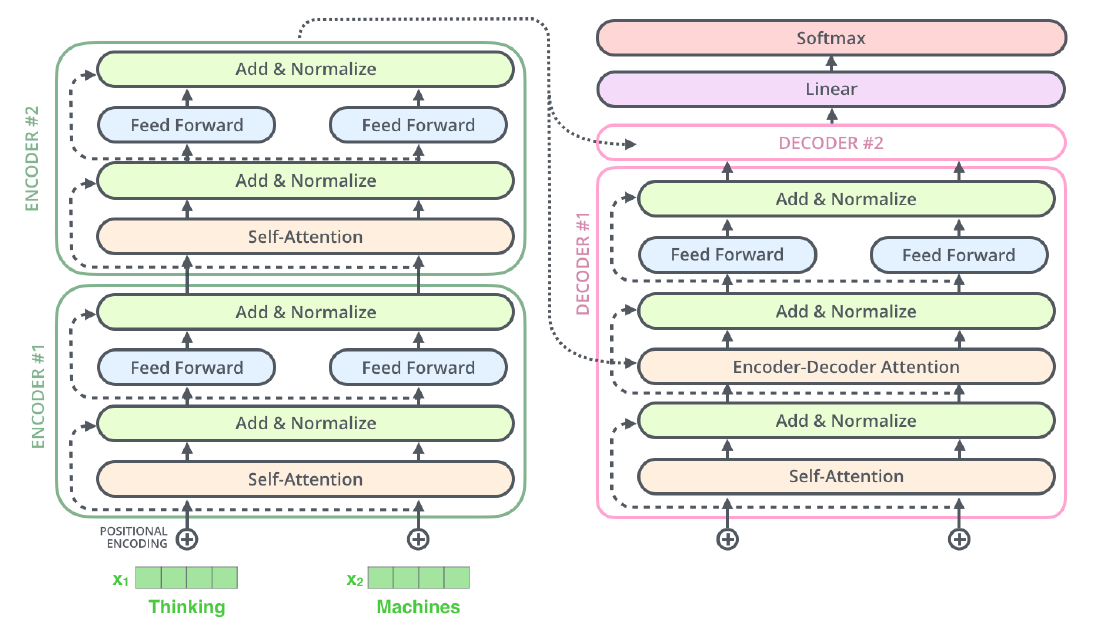
\includegraphics[width=0.75\textwidth]{transformer.png}
\end{figure}

The decoder of a Transformer is similar to the encoder, with the addition of encoder-decoder attention layers. The decoder takes a prefix of an output sentence as input and predicts the next word until it generated an \b{end token} as output. Its self-attention layer is only allowed attend to earlier predictions in the output sentence, the future positions are masked.

\subsection{Limitations of Attention}
\begin{itemize}
    \item The complexity of storing the self-attention matrix of an input of length \f{n} is \f{O(n^2)}.
    \item Attention can not deal with arbitrary long inputs. The input has to be split into segments.
    \item Low inductive bias.
    \item Need to be very large to reach good performance.
\end{itemize}